\section{Echtzeit Polygon Rekonstruktion} \label{sec:polygon_reconstruction}

Das zweite Rekonstuktions basierte Überlagerungsverfahren basiert in diesem Kapitel auf dem aktuellen Forschungsstand der Echtzeit Rekonstruktion und soll folgenden Absätzen näher beschrieben werden. Die 3D Rekonstruktion ist bereits ein etabliert Forschungsgebiet in der Computer Grafik und gewinnt, auf Grund von kostengünstigen Consumer Tiefensensoren, wie die Microsoft Kinect, Asus Xtion oder Structure \citep{Struc48:online}, zunehmend an Bedeutung. Dabei wird sich immer mehr auf die Echtzeit Rekonstruktion konzentriert, da diese Geräte in der Lage sind, Tiefeninformationen, zwar mit leichten Messfehlern aber in Echtzeit, zu liefern. \citet{niessner2013real} erwähnen an dieser Stelle zudem den möglichen Einsatz für Augmented Reality:

\begin{quote}
\enquote{The ability to obtain reconstructions
in real-time opens up various interactive applications including:
augmented reality (AR) where real-world geometry can be fused
with 3D graphics and rendered live to the user; ...} \citep{niessner2013real}
\end{quote}

Die Herausforderung in der Echtzeit Rekonstruktion liegt dabei in der möglichst performanten Fusion von mehreren überlagernden Depth Maps. Hieraus soll eine möglichst detailierte Repräsentation der echten Umgebung generiert werden, welche sich im Idealfall stetig verbessert. Diese Problemstellung unterscheidet sich dabei von herkömmlichen Rekonstruktionsverfahren wie die von \citet{hoppe1992surface} und der Poission Rekonstruktion von \citet{kazhdan2006poisson}. Aktuelle Verfahren nutzen verschiedenste optimierte Datenstrukturen, welche zudem durch den Einsatz von entsprechenden GPU Implementierungen beschleunigt werden können. Dennoch spielt die Gegenüberstellung von Detailgrad, der Skalierung und Geschwindigkeit stets eine große Rolle. \citet{niessner2013real} \\

Bekannte Verfahren wie KinectFusion \citep{newcombe2011kinectfusion}, ein SLAM Verfahren von \citet{bylow2013real} oder DynamicFusion \citep{newcombe2015dynamicfusion} nutzen die \enquote{Truncated Signed Distance Function}, kurz TSDF, zur Speicherung und Migration der Oberflächeninformation mehrerer Depth Maps. Das Verfahren von \citet{niessner2013real} erweitert diesen Ansatz mit einem effizienten Spatial Hashing Verfahren, um die Zugriffszeiten und Speicherverbrauch zu minimieren. Darüber hinaus nimmt das Verfahren Chisel von \citep{Klingensmith_2015_7924} diese Vorzüge auf und kombiniert TSDF mit \enquote{visual-inertial odometry}, der Trackingtechnologie von Project Tango. In den folgenden Absätzen werden die Mechanismen hinter TSDF, dem räumlichen Hashing und den Vorzügen von Chisel näher erläutert. Außerdem soll auch noch auf das Rendering der TSDF Oberfläche durch Marching Cubes eingegangen werden, welches in Chisel verwendet wird. \\


\subsection{Truncated Signed Distance Function}

Bei der von \citet{curless1996volumetric} vorgestellten räumlichen Repräsentation von Oberflächen, Truncated Signed Distance Function (TSDF), wird der Raum in Voxel einer gewünschten Auflösung unterteilt. Anders als Occupancy Maps, in denen die Voxel als sichtbar oder unsichtbar markiert werden, werden bei TSDF in den Voxeln die jeweiligen Entfernungen zur nächsten Oberfläche angegeben. Wichtig dabei ist das Vorzeichen, welches angibt, ob sich ein Voxel innerhalb oder außerhalb eines Objektes befindet. Abbildung \ref{fig:tsdf} zeigt unter a) die Ergebnisse mit Occupancy Maps und in b) die Voxel von TSDF. \citep{curless1996volumetric} \\

Gefüllt wird die Repräsentation durch die Depth Maps und der entsprechenden Kameraposition, die im Fall von Project Tango bereits gegeben ist. So wird für jede Tiefeninformation ein Strahl ausgehend von der Kameraposition generiert, der die durchgeschnittenen Voxel aktualisiert. Der Stahl ist dabei von der Länge begrenzt, um die zu aktualisierenden Voxel zu minimieren und zudem keine Oberflächen zu aktualisieren, die sich weiter hinter der gefundenen Oberfläche befindet. Dieses Vorgehen ist in Abbildung \ref{fig:tsdf} c) zu erkennen. \citep{Compu66:online} \\

\begin{figure}
  \centering
	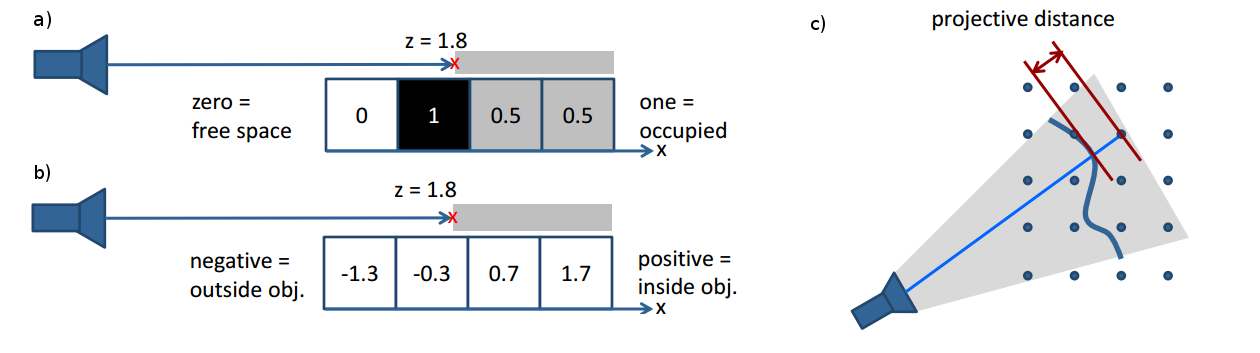
\includegraphics[width=1.0\textwidth]{content/images/methods/tsdf.png} 
  \caption{a) Beispielhafte Voxel Füllung von Occupancy Maps; b) Beispielhafte Voxel Füllung durch TSDF; c) Exemplarische 2D Darstellung der Oberfläche mit entsprechenden Strahlensatz für die TSDF. Übernommen von \citet{Compu66:online}}
  \label{fig:tsdf}
\end{figure}

Der Vorteil dieser Repräsentation liegt darin, dass die konkreten Oberflächeninformationen, anders als bei der Diskretisierung von Occupancy Maps, nicht verloren gehen. Das heißt, dass trotz einer gröberen Voxel Struktur stets der Nulldurchgang rekonstruiert werden kann. Neben der Entfernung zur nächsten Oberfläche wird zusätzlich noch ein Gewichtungswert in jedem Voxel gespeichert. Das ermöglicht es leichtes Rauschen durch einfache Mittelung zu unterdrücken und die Oberfläche optimiert sich somit bei jeder Aktualisierung der Voxel. \citep{Compu66:online}\\

\citet{hoppe1992surface} nutzen in Ihrem Rekonstruktionsverfahren auch die hier beschriebene TSDF. Jedoch bestimmen sie für jeden festgehaltenen Punkt der Pointcloud die umliegenden Nachbarn, um eine Tangentialebene zu ermitteln, von der aus die auf der Normalen liegenden Voxel mit der entsprechenden Distanz aktualisiert werden. Für die Echtzeitrekonstruktion ist dieses Vorgehen jedoch zu komplex. Hier werden die Voxel nicht anhand der exakten euklidischen Distanz aktualisiert, sondern es wird mit Hilfe des Raycastings, ausgehend von der Tiefenkamera, eine projizierte Distanz als Approximation verwendet. \citep{Compu66:online}

\subsection{Spatial Hashing}

Das Problem der Echtzeit Rekonstruktion ist wie bereits angesprochen der Kompromiss zwischen dem Detailgrad, der Skalierung der zu rekonstruierenden Szene und der Performance der Rekonstruktion. Auch die TSDF Repräsentation ist sehr speicherintensiv und benötigt für die zu scannende Szene reservierten Speicher, der auf mobilen Endgeräten nur begrenzt verfügbar ist. Daher muss auch für größere Rekonstruktionen oder Rekonstruktionen unbekannter Größe ein dynamischer Ansatz gefunden werden. \citet{Klingensmith_2015_7924} erwähnt dazu, dass einige Verfahren Octrees einsetzen, die zwar äußerst dynamisch sind, jedoch einen deutlichen Nachteil hinsichtlich der Zugriffszeiten auf die Voxel bergen. \\

\begin{figure}[h]
  \centering
	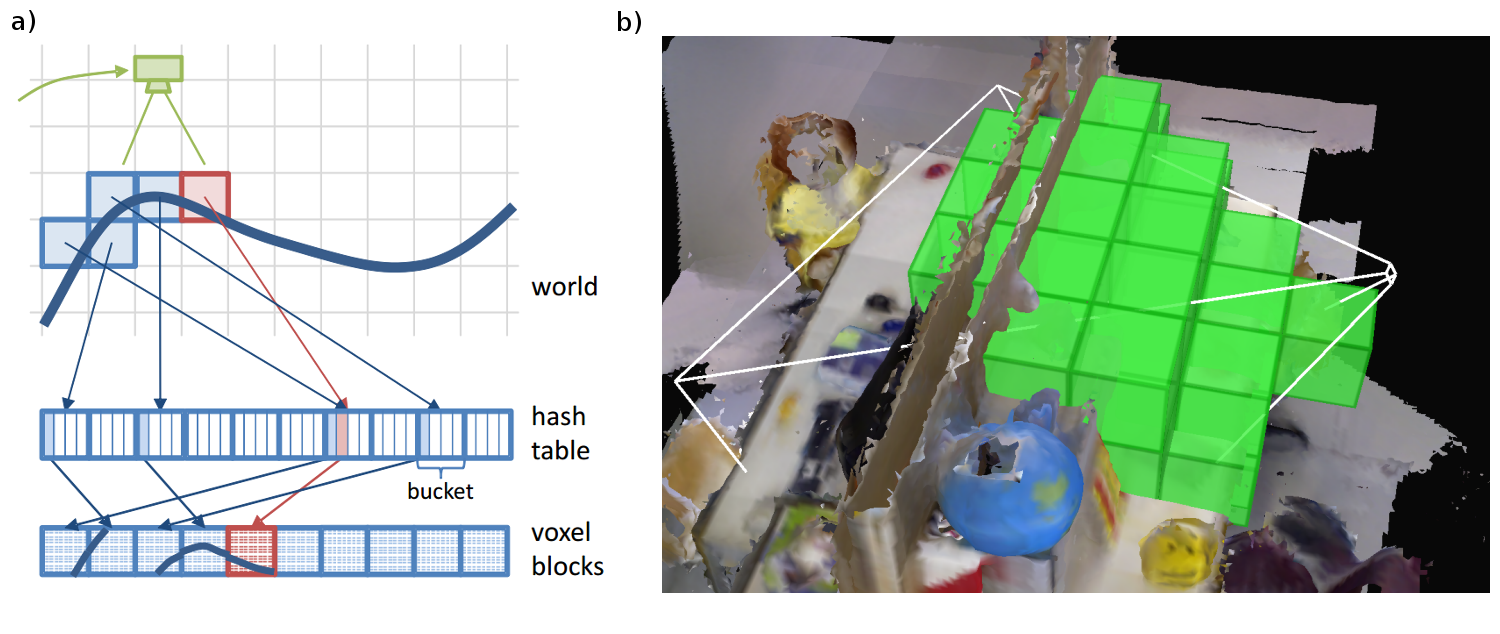
\includegraphics[width=1.0\textwidth]{content/images/methods/hashing.png} 
  \caption{a) Voxel Hashing Datenstruktur. Übernommen von \citet{niessner2013real} b) Darstellung der relevanten Voxel Chunks für die Aktualisierung. Übernommen von \citet{Klingensmith_2015_7924}}
  \label{fig:hashing}
\end{figure}

\citet{niessner2013real} führen daher eine zwei-Ebenen Struktur ein, die auf der zweiten Ebene eine Menge von Voxel räumlich zusammenfassen. Diese werden hier Chunks genannt. Auf der ersten Ebene können diese Chunks in einer Hash Tabelle räumlich mit einer Hashfunktion identifiziert werden. Das ermöglicht somit einen nahezu direkten Zugriff auf räumliche Voxel und ermöglicht es zudem Chunks dynamisch zu allokieren. Als Hash der Chunkposition \(x\), \(y\) und \(z\) wird die folgende Hashfunktion aus Gleichung \ref{eq:spatial_hash} verwendet. Bei den Variablen \(p_1\), \(p_2\) und \(p_3\) handelt es sich um willkürlich hohe Primzahlen und \(n\) entspricht der Größe der Hash Tabelle. 

\begin{equation}\label{eq:spatial_hash}
H(x,y,z) = (x * p_1 \oplus y * p_2 \oplus z * p_3) \mod n
\end{equation}

\subsection{Marching Cubes}

Die meisten Echtzeit Rekonstruktionen durch TSDF wie KinectFusion sind GPU Umsetzungen, die daher die Möglichkeit besitzen ein hardwarebeschleunigtes Rendering durch Raycasting durchzuführen. Das Verfahren Chisel von \citet{Klingensmith_2015_7924}, welches eine reine CPU Umsetzung ist, nutzt hingegen einen indirekten Weg zum Rendering durch die Marching Cubes Triangulation. \\

\begin{figure}[h]
  \centering
	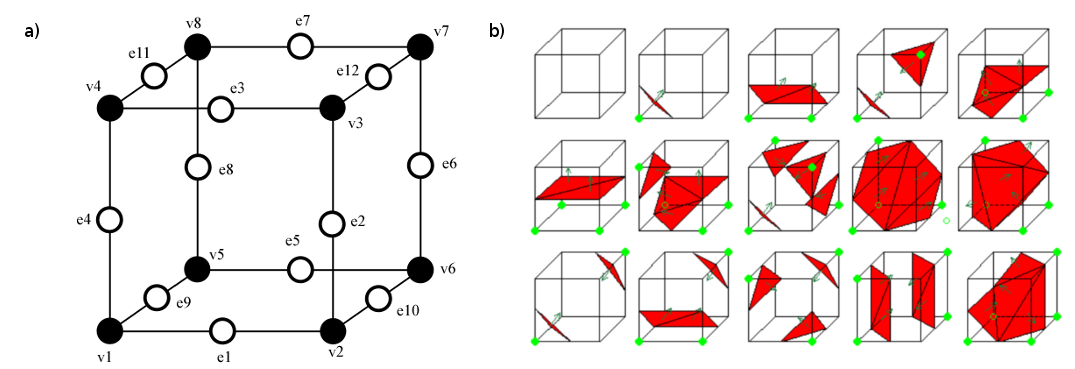
\includegraphics[width=1.0\textwidth]{content/images/methods/marchingcubes.png} 
  \caption{a) Marching Cubes Voxel Repräsentation mit den Ecken und den Kantenschnittpunkten b) Die 15 möglichen 3D Polygon Varianten. Übernommen von \citet{MarchingCubes:online}}
  \label{fig:marchingcubes}
\end{figure}

Marching Cubes nach \citet{lorensen1987marching} ist ein Algorithmus um aus einer, als Voxel repräsentierten, Isofläche Polygone zu bestimmen, die dieser Fläche möglichst nah kommt. Hierzu werden zu jedem Voxel die Ecken \(v1\) bis \(v8\) anhand der Nachbarvoxel und des Distanzwertes untersucht, ob sie innerhalb oder außerhalb eines Objektes liegen. Zusätzlich werden zu jeder Kante auf dem Voxel, wenn ein Schnitt der Isofläche existiert, die Schnittpunkte auf den Kanten \(e1\) bis \(e12\) bestimmt. Abbildung \ref{fig:marchingcubes} a) zeigt die Ecken und Kantenschnittpunkte eines Voxels. \\

Je nach binärer Gewichtung der Ecken können hiernach aus einem Katalog von 256 Varianten die Polygone nachgeschlagen werden. Inhalt des Katalogs sind die Indizes der Kantenschnittpunkte, aus denen Polygone generiert werden können. Alle diese 256 Varianten können auf 15 verschiedene Fälle zurückgeführt werden, die sich nur in Rotation oder Symmetrie unterscheiden. Die 15 Varianten sind in Abbildung \ref{fig:marchingcubes} b) zu finden. \citep{MarchingCubes:online} \\

\subsection{Chisel mit Space Carving}

Das Bereits erwähnte Verfahren Chisel von \citet{Klingensmith_2015_7924} verwendet alle zuvor erwähnten Techniken der TSDF, spatial Hashing und der Marching Cubes Überführung. Sie sprechen dabei von einem \enquote{dynamic spatial-hashed truncated distance field}. Das für den mobilen Einsatz optimierte Verfahren ist in der Lage eine Echtzeitrekonstruktion von Räumen von bis zu \(300 m^2\) mit einem Detailgrad von zwei bis drei Zentimetern zu erstellen. Zudem können neben Tiefeninformationen auch gefärbte Pointclouds verarbeitet werden, wodurch ein gefärbtes Mesh generiert werden kann. \citep{Klingensmith_2015_7924}\\

Zusätzlich erweitern sie den TSDF Algorithmus um die \enquote{space carving} Funktionalität. Sie betrachten dabei den Strahl von der Kamera zur Oberfläche als eine Art Constraint, in dem alle durchstoßenden Voxel bis zur Oberfläche eine negativen Wert beinhalten müssen. Ist das nicht der Fall, so wird ein Voxel außerhalb der inneren Begrenzung auf den leeren Ursprungswert gesetzt. Im Pseudocode aus Listing \ref{lst:chisel} wird das Verhalten näher erläutert. Diese Verbesserung führt dazu, dass die Rekonstruktion bei stark rauschenden Tiefeninformationen, besonders an Objektkanten, deutlich verbessert wird. Außerdem ist das Verfahren hiermit in der Lage dynamische Änderungen in der Umgebung zu detektieren und neue Oberflächen entsprechend zu aktualisieren. So beeinflussen zum Beispiel sich im Bild bewegen Personen nur kurz die Voxel der TSDF. \citep{Klingensmith_2015_7924}\\

\begin{lstlisting}[mathescape,caption=Chisel TSDF Algorithmus, label=lst:chisel, float=htbp]
Eingabe: Pointcloud $C$, Kameratransformation $P_{cam}$, 
         Strahlenbegrenzung $t$

für jeden Tiefenwert $\vec{p}$ aus $C$
    bestimme die Oberflächenposition $\vec{z}$ aus $\vec{p}$ und $P_{cam}$
    bestimme einen Strahl $\vec{r}$ aus $\vec{z}$ und $P_{cam}$
    bestimme den Begrenzungsbereich $t_{vor}$, $t_{nach}$ mit $t$ um $\vec{z}$ auf $\vec{r}$
    # space carving
    für jeden Voxel $v$ zwischen Kamera und $t_{vor}$
        wenn die Distanz im Voxel negativ ist
            setze Voxel zurück
    # normale TSDF Bestimmung
    für jeden Voxel $v$ zwischen $t_{vor}$ und $t_{nach}$
        bestimme die Voxeldistanz zu $z$
        setze das Gewicht w des Voxels $v$
\end{lstlisting}

Neben space carving wurden zudem eine variable Strahlenbegrenzungen und Gewichtungen der Voxel abhänig von der jeweils aufgenommenen Tiefe implementiert. Diese Funktion berücksichtigt die Varianzen von Messungenauigkeiten des Sensors, die bei größerer Entfernung der Oberfläche zum Tiefensonsor zunehmen können. \citep{Klingensmith_2015_7924}

\textbf{TODO:} DARSTELLUNG DES STRAHLS, DER KAMERA UND DER OBERFLÄCHE ZUR VERSTÄNDNIS DES ALGORITHMUS